% The bundled acmart.cls (v1.88) loads hyperxmp before hyperref, which the current
% hyperxmp rejects ("hyperref must be loaded before hyperxmp"), so template.tex itself
% doesn't build on TeX Live 2026. acmart uses no hyperxmp feature: mark it as loaded.
\expandafter\def\csname ver@hyperxmp.sty\endcsname{}
\documentclass[sigconf]{acmart}
\settopmatter{printacmref=false, printccs=false, printfolios=true}
\renewcommand\footnotetextcopyrightpermission[1]{}
\acmConference[ComPar 26/27]{ComPar 26/27 Project 1}{November 2026}{NOVA FCT, Portugal}

\usepackage{booktabs} % For formal tables
\usepackage{tabularx}
\usepackage{enumitem}
\setlist{nosep, leftmargin=*}
\usepackage{pgfplots}
\usepackage{pgfplotstable}
\pgfplotsset{compat=1.18}
\usetikzlibrary{positioning, arrows.meta, calc}

% Keep only the rows of a CSV whose column #1 equals #2 (env = docker / local).
\pgfplotsset{
  discard if not/.style 2 args={
    x filter/.append code={
      \edef\tempa{\thisrow{#1}}%
      \edef\tempb{#2}%
      \ifx\tempa\tempb\else\def\pgfmathresult{inf}\fi
    }
  }
}

% Every number in this report comes from experiments/LOG.md (the run-ids are there,
% section by section) or from experiments/analysis/*.csv (Figure 4 and Table 7).
\newcommand{\mib}{\,MiB}
\newcommand{\s}{\,s}
\setlength{\emergencystretch}{2em}
\definecolor{hot}{RGB}{196,110,40}
\tikzset{
  box/.style={draw, rounded corners=2pt, align=center, font=\scriptsize,
              minimum height=0.62cm, text width=2.35cm, inner sep=1.5pt},
  hotbox/.style={box, draw=hot, fill=hot!12, thick},
  note/.style={font=\scriptsize\itshape, text=hot, align=center},
  flow/.style={-{Stealth[length=4pt]}},
}

\begin{document}
\title{SHARD: Measurement-Driven Performance Engineering of a Spark Pipeline over NYC Taxi Trips}

\author{Radesh Govind}
\email{p215604@campus.fct.unl.pt}
\affiliation{\institution{NOVA FCT}\city{Caparica}\country{Portugal}}

\begin{abstract}
This report studies the run time of a Spark pipeline of five operations over 48.7 million New
York taxi trips from 2025, on a laptop and on a simulated cluster of workers running on that
same laptop. Measuring each part showed two delays. \emph{First}, the same files were read five
times, once per operation (about three fifths of the run time). Keeping the cleaned trips in
memory had the opposite effect: the pipeline took 32\,\% to 42\,\% longer, because building
the copy cost more than the reading it saved, and on the cluster the copy did not fit in
memory. \emph{Second}, the operation that finds unusual fares regrouped every trip across tasks,
sorted it and partly wrote it to disk (about one sixth). Letting each task first sum its own
trips made that operation about two fifths faster, and the whole pipeline 16\,\% faster on the
laptop and 9\,\% on the cluster. A third change, to one join, gave no measurable gain. The run
time grows much less than the data, and adding workers on one laptop does not reduce it; both
are traced to measured causes.
\end{abstract}

\keywords{Apache Spark, performance engineering, shuffle, broadcast join, Amdahl's law}

\maketitle

% =====================================================================
\section{Introduction}

Many programs must process more data than one processor can handle quickly. Spark is a tool
for this: it splits a data job into tasks that run on many processors at the same time. A
program that reads data, computes results from it and writes them to files is a
\emph{pipeline}. This report studies one pipeline and asks how to make it faster.

\textbf{The data.} The pipeline works on the trips of the New York yellow taxis in
2025~\cite{tlcdata}: 48,722,602 trips, one row per trip, in 12 monthly Parquet files
(829,973,299\,B). Each trip has its start and end time, pickup and drop-off zone, passengers,
distance, fare and payment type. Valid zone numbers are 1--263; a lookup table of 265 rows gives
each zone its borough. After five validity checks (e.g.\ a fare above zero), 43,599,832 trips
remain.

\textbf{The five operations.} Table~\ref{tab:ops} lists the five results, each with the
question it answers and the reason it takes time. O1 and O3 were chosen from the optional
operations because they stress two different costs: O1 regroups every trip for its group
statistics, and O3 depends on how Spark chooses to execute a join.

\begin{table*}[t]
\caption{The five operations. M = required by the assignment, O = optional, chosen by the author.}
\label{tab:ops}
\footnotesize
\begin{tabularx}{\textwidth}{@{}>{\raggedright\arraybackslash}p{1.9cm}>{\raggedright\arraybackslash}p{5.6cm}X@{}}
\toprule
Operation & The question it answers & Why it takes time \\
\midrule
M1 cleaning & Which trips are valid? Five checks, e.g.\ a fare above zero; count the trips that fail each check. & Like every operation, it reads and checks the whole year. \\
M2 demand by hour & How many trips start in each borough, weekday and hour, and what are their average fare, duration and distance? & One pass over all trips, which each task first sums up locally. \\
M3 zone statistics & How does each zone change from month to month, and which months are unusual for it? & It first sums all trips into one row per zone and month (3,083 rows); its window functions on that small table are cheap (0.56\s{} laptop, 1.0\s{} cluster). \\
O1 unusual fares & Which trips cost far more per kilometre than similar trips (same pickup zone, same hour), i.e.\ above the group's mean + 3$\sigma$? & The mean and $\sigma$ of each group are computed with a window, so the trips of a group must meet in one task: every trip is regrouped across tasks (a \emph{shuffle}), sorted, and partly written to disk. The largest group has 169,582 trips. \\
O3 demand features & How busy is each zone in each hour, compared with its usual level at that weekday and hour, and with the same hour four weeks earlier? & The counts per zone and hour (2,303,880 rows) are joined with a copy shifted by four weeks (672 hours). Spark picks the join method from a size estimate~\cite{armbrust2015}: 9.58\,MB on a one-month run, just under the 10.49\,MB limit for copying a table to every task; 122.44\,MB on the year, where Spark therefore regroups and sorts both sides. \\
\bottomrule
\end{tabularx}
\end{table*}

\textbf{The method.} Each improvement follows the loop of Figure~\ref{fig:loop}: measure where
the time goes, state a hypothesis about the cause, change one thing, and measure again. A change
is kept only if the new measurement is better. Sections 3 and 4 follow these steps; Section~5
tests the final program with more data and more workers.

\begin{figure}[h]
\centering
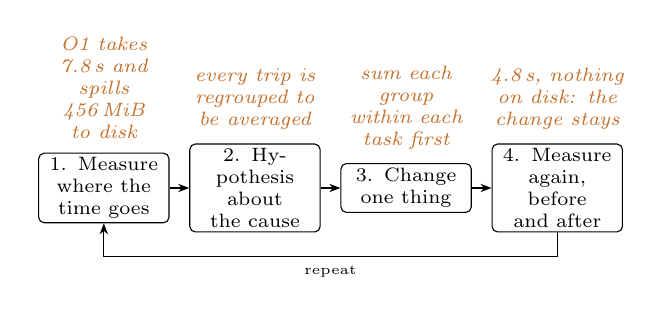
\begin{tikzpicture}[node distance=0.25cm]
\node[box, text width=1.55cm] (m) {1. Measure\\where the time goes};
\node[box, text width=1.55cm, right=of m] (h) {2. Hypothesis\\about the cause};
\node[box, text width=1.55cm, right=of h] (c) {3. Change\\one thing};
\node[box, text width=1.55cm, right=of c] (a) {4. Measure again,\\before and after};
\draw[flow] (m) -- (h); \draw[flow] (h) -- (c); \draw[flow] (c) -- (a);
\draw[flow] (a.south) -- ++(0,-0.3) -| node[pos=0.25, below, font=\tiny] {repeat} (m.south);
\node[note, text width=1.7cm, above=0.05cm of m] {O1 takes 7.8\s{} and spills 456\mib{} to disk};
\node[note, text width=1.7cm, above=0.05cm of h] {every trip is regrouped to be averaged};
\node[note, text width=1.7cm, above=0.05cm of c] {sum each group within each task first};
\node[note, text width=1.7cm, above=0.05cm of a] {4.8\s, nothing on disk: the change stays};
\end{tikzpicture}
\caption{The measure-and-improve loop, with the example of Section~4.2 (laptop).}
\label{fig:loop}
\end{figure}

% =====================================================================
\section{Pipeline}

The pipeline works in four steps: (1) read the 12 monthly files; (2) check the trips against
the five rules of M1 (M1 counts the failures, the other operations remove those trips);
(3) compute the result of each operation; (4) write the results to files. The operations run
one after the other and do not share data, so each one reads the whole year again.

\textbf{How the program is written.} The program is written in Kotlin, using Spark's DataFrame
API on the Java virtual machine (JVM). Every step is a built-in Spark expression, with no
user-defined functions; DataFrame code and SQL are optimised by the same engine
(Catalyst~\cite{armbrust2015}), and the DataFrame form is checked by the compiler. A program
option (\texttt{--skip-opts}) switches each tested change off, so old and new versions run from
one build. No Spark configuration property was changed.

\textbf{One plan as an example.} Figure~\ref{fig:plan} shows the final plan of the
unusual-fare operation (O1) as Spark ran it: (a) at first, (b) after the change of
Section~4.2.

\begin{figure*}[t]
\centering
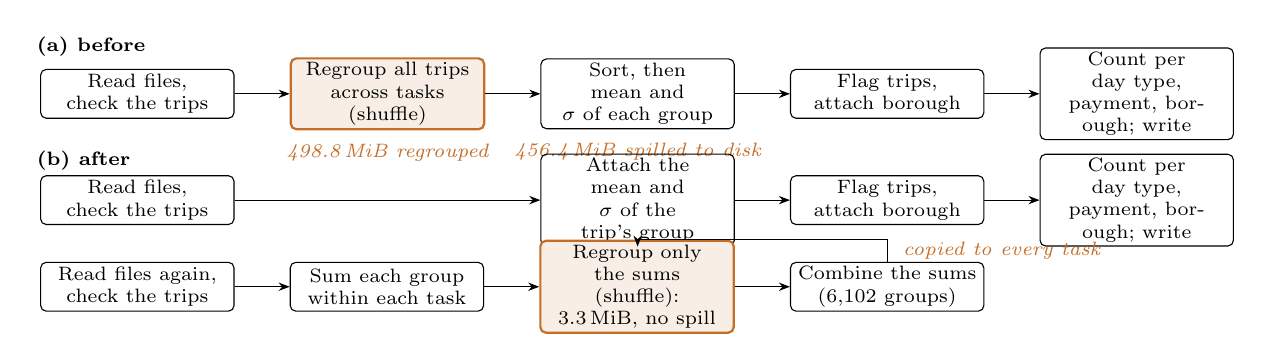
\begin{tikzpicture}[node distance=0.7cm]
\node[font=\scriptsize\bfseries, anchor=west] at (-1.4,0.6) {(a) before};
\node[box] (a1) at (0,0) {Read files,\\check the trips};
\node[hotbox, right=of a1] (a2) {Regroup all trips\\across tasks (shuffle)};
\node[box, right=of a2] (a3) {Sort, then mean and\\$\sigma$ of each group};
\node[box, right=of a3] (a4) {Flag trips,\\attach borough};
\node[box, right=of a4] (a5) {Count per day type,\\payment, borough; write};
\foreach \x/\y in {a1/a2,a2/a3,a3/a4,a4/a5} \draw[flow] (\x) -- (\y);
\node[note, below=0.05cm of a2] {498.8\mib{} regrouped};
\node[note, below=0.05cm of a3] {456.4\mib{} spilled to disk};

\node[font=\scriptsize\bfseries, anchor=west] at (-1.4,-0.85) {(b) after};
\node[box] (b1) at (0,-1.35) {Read files,\\check the trips};
\node[box] (b3) at ($(a3)+(0,-1.35)$) {Attach the mean and\\$\sigma$ of the trip's group};
\node[box, right=of b3] (b4) {Flag trips,\\attach borough};
\node[box, right=of b4] (b5) {Count per day type,\\payment, borough; write};
\draw[flow] (b1) -- (b3); \draw[flow] (b3) -- (b4); \draw[flow] (b4) -- (b5);
\node[box] (c1) at (0,-2.45) {Read files again,\\check the trips};
\node[box, right=of c1] (c2) {Sum each group\\within each task};
\node[hotbox, right=of c2] (c3) {Regroup only the sums\\(shuffle): 3.3\mib, no spill};
\node[box, right=of c3] (c4) {Combine the sums\\(6,102 groups)};
\foreach \x/\y in {c1/c2,c2/c3,c3/c4} \draw[flow] (\x) -- (\y);
\draw[flow] (c4.north) -- ++(0,0.28) -| (b3.south);
\node[note, anchor=west] at ($(c4.north)+(0.08,0.14)$) {copied to every task};
\end{tikzpicture}
\caption{Final plan of the unusual-fare operation (O1), 2025, laptop, before (a) and after (b)
the change; simplified from the plans Spark recorded. Read each row left to right; the
outlined boxes are where data is regrouped across tasks. After the change only small sums are
regrouped, and the trips are read twice: the lower row runs first, and its result is copied to
every task of the upper row.}
\label{fig:plan}
\end{figure*}

% =====================================================================
\section{Profiling and Baseline}

The first step of the loop is to measure the pipeline as it is. These first measurements are
the \emph{baseline}, and every later change is compared with them.

\textbf{On which machines?} The measurements ran on a laptop and on a simulated cluster
(Table~\ref{tab:machines}). A cluster is a group of computers, called workers, that share a
job. In the simulated cluster the workers are containers on the same laptop and share its
hardware.

\begin{table}[h]
\caption{The two test machines.}
\label{tab:machines}
\footnotesize\setlength{\tabcolsep}{4pt}
\begin{tabularx}{\columnwidth}{@{}l>{\raggedright\arraybackslash}X>{\raggedright\arraybackslash}X@{}}
\toprule
 & Laptop & Simulated cluster \\
\midrule
what it is & Spark directly on the laptop & Spark master and workers in Docker containers on the laptop, linked by a virtual network \\
hardware & Apple M5, 10 cores (4 performance, 6 efficiency), 24\,GB & the same laptop, via a VM of 10 CPUs and 11.73\,GiB \\
workers & one process, 10 cores & 2 workers of 2 cores (2--5 in Section~5), 1024\,MiB each \\
software & \multicolumn{2}{l}{Spark 4.2.1 and Java 21 on both} \\
\bottomrule
\end{tabularx}
\end{table}

\textbf{How was the time measured?}
\begin{itemize}
\item \emph{Recorded:} a Kotlin version of the Lab~3 profiling tool~\cite{compar2026} records
each operation's run time, its stage metrics (data regrouped, spilled) and the final plans. The
run time $T$ is the sum of the five operations, without the start of Spark.
\item \emph{Alternation:} the laptop is not a steady machine. Whole sessions differed by up to
about 40\,\% on the same code (in one, Low Power Mode was on), so the old and new versions
always ran in alternation, in one session, from one build. A warm-up run was discarded, and
medians are reported.
\end{itemize}

\textbf{What did the measurements show?} Table~\ref{tab:baseline} gives the baseline: 25.94\s{}
on the laptop and 34.77\s{} on the simulated cluster.
\begin{itemize}
\item The unusual-fare operation (O1) was the slowest (7.79\s{} on the laptop).
\item It was also the only operation that spilled data to disk (456.4\mib).
\item The tasks spent 71\,\% (laptop) and 88\,\% (cluster) of their run time computing on a
processor, and 3.5\,\% and 5.4\,\% in garbage collection, so reading from disk and memory
cleanup were not the main costs.
\end{itemize}

\begin{table}[h]
\caption{Baseline (before) and final pipeline (after), 2025, 7 alternating pairs, medians in s
(ranges in Table~\ref{tab:summary}).}
\label{tab:baseline}
\footnotesize\setlength{\tabcolsep}{3pt}
\begin{tabular}{@{}lrrrr@{}}
\toprule
 & \multicolumn{2}{c}{Laptop, 10 cores} & \multicolumn{2}{c}{Cluster, 2$\times$2 cores} \\
 & before & after & before & after \\
\midrule
whole pipeline $T$ & \textbf{25.94} & \textbf{21.70} & \textbf{34.77} & \textbf{31.74} \\
M1 / M2 / M3 & 4.52/3.00/5.14 & 4.37/2.86/4.93 & 5.86/4.50/7.21 & 5.86/4.33/7.56 \\
O1 / O3 & 7.79/5.31 & 4.51/5.02 & 9.18/7.67 & 5.43/8.17 \\
regrouped (MiB) & 656.9 & 161.4 & 650.0 & 153.9 \\
spilled to disk (MiB) & 456.4 & 0 & 431.7--432.1 & 0 \\
\bottomrule
\end{tabular}
\end{table}

To see which parts decide the total time, Figure~\ref{fig:shares} splits the baseline's
critical path. The five reading stages (each also checks the trips and starts its operation)
took about three fifths; O1's sort-and-average step about one sixth. These shares come from an
earlier session whose times were about 1.6 to 1.7 times longer (41.19\s{} and 58.28\s), with
the same plans, data volumes and task counts.

\begin{figure}[h]
\centering
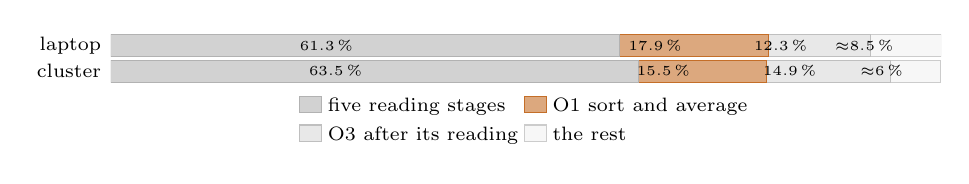
\begin{tikzpicture}
\begin{axis}[
  xbar stacked, width=\columnwidth, height=2.2cm, bar width=8pt,
  xmin=0, xmax=100, axis x line=none, axis y line*=left, y axis line style={draw=none},
  ytick=data, symbolic y coords={cluster, laptop}, enlarge y limits=0.45,
  tick label style={font=\scriptsize}, major tick length=0pt,
  nodes near coords={\pgfmathprintnumber[fixed, precision=1]{\pgfplotspointmeta}\,\%},
  nodes near coords style={font=\tiny},
  every node near coord/.append style={anchor=east, xshift=-1pt},
  legend style={font=\scriptsize, at={(0.5,-0.08)}, anchor=north, legend columns=2, draw=none},
  legend cell align=left,
]
\addplot[fill=gray!35, draw=gray!60] coordinates {(61.3,laptop) (63.5,cluster)};
\addplot[fill=hot!60, draw=hot] coordinates {(17.9,laptop) (15.5,cluster)};
\addplot[fill=gray!18, draw=gray!50] coordinates {(12.3,laptop) (14.9,cluster)};
\addplot[fill=gray!6, draw=gray!40, nodes near coords={$\approx$\pgfmathprintnumber{\pgfplotspointmeta}\,\%}] coordinates {(8.5,laptop) (6,cluster)};
\legend{five reading stages, O1 sort and average, O3 after its reading, the rest}
\end{axis}
\end{tikzpicture}
\caption{Where the baseline run time went (share of the critical path, earlier session).}
\label{fig:shares}
\end{figure}

\textbf{Suspected causes.} Table~\ref{tab:causes} lists the six suspected causes, each with
the most it could save. Section~4 tests three; a fourth was dropped before measuring.

\begin{table*}[t]
\caption{Suspected causes, evidence, and the most each could save (share of the baseline run
time, laptop / cluster).}
\label{tab:causes}
\footnotesize
\begin{tabularx}{\textwidth}{@{}l>{\raggedright\arraybackslash}p{5.2cm}Xl@{}}
\toprule
 & Suspected cause & Evidence, and what happened & Saves up to \\
\midrule
1 & The input is read again for each operation & 829,973,299\,B and 48,722,602 records read by each of the five operations; nothing kept in memory. Tested: change 1. & 37.8 / 38.0\,\% \\
2 & O1 regroups, sorts and averages all trips & 498.8\mib{} regrouped, 456.4\mib{} spilled; tasks of even length (longest / median 1.03). Tested: change 2. & 17.9 / 15.5\,\% \\
3 & Idle cores in the last round of each reading & One task per file: 12 tasks on 10 cores (laptop), 10 on 4 (cluster). Not tested. & 13.1 / 12.7\,\% \\
4 & A text pattern extracted from the file path of every row (M1, M3) & M1 and M3 read more slowly than the others, but they also compute more. Not tested. & up to 11\,\% \\
5 & O3 computes the same joined table twice & Two stages each read the same 32.9\mib. Dropped: keeping it in memory grew O3 from 76 to 855 tasks (plan run). & 5.2 / 6.4\,\% \\
6 & O3's four-week join regroups and sorts both sides & 64.2\mib{} regrouped again on one side, 24.5\mib{} on the other. Tested: change 3. & 3.2 / 4.9\,\% \\
\bottomrule
\end{tabularx}
\end{table*}

% =====================================================================
\section{Optimisation Study}

Each change was tested alone, switched by the program option and measured as in Section~3.
Every version printed the same results (O1's internal averages agree to within $10^{-12}$
relative). Table~\ref{tab:summary} lists every number.

\subsection{Change 1 (cause 1): keep the cleaned trips in memory --- undone}
\textbf{Bottleneck.} Five operations read and check the whole year: about three fifths of the
baseline. \textbf{Hypothesis.} If the cleaned trips are kept after the first use, the later
operations need not read the files again. \textbf{Change.} After cleaning, the trips are
stored in memory (and on disk when memory is full) and released after the last operation.
\textbf{Data.} The later operations read nothing from the files, as intended (0 records instead
of 48,722,602). \textbf{Time.} The pipeline took 32\,\% longer on the laptop (25.54 $\to$
33.61\s) and 42\,\% longer on the cluster (34.21 $\to$ 48.64\s). \textbf{Reason.} Building
the copy cost more than the reading it saved: M2, which fills the copy, became 10.11\s{}
(laptop) and 15.24\s{} (cluster) slower, only M3 gained (3.61 and 4.68\s), and O3 became slower
because it now read the copy twice. On the cluster the copy (4,828--5,689\mib) did not fit in
the workers' storage memory (434\mib{} each), so it lived entirely on disk. \textbf{Verdict.}
Undone. Keeping data in memory pays only if the copy fits and costs less to build than the
reading it saves.

\subsection{Change 2 (cause 2): sum first, then attach --- kept}
\textbf{Bottleneck.} O1 needs the mean and $\sigma$ of the fare per kilometre of each group
(one pickup zone in one hour). With a window, the trips of a group must meet in one task, so
all 43.6 million trips were regrouped (498.8\mib), sorted and partly spilled to disk
(456.4\mib): about one sixth of the run time. \textbf{Hypothesis.} If each task first sums its
own trips per group, only small sums travel (at most 6,312 groups per task), and the sort
disappears. \textbf{Change.} The sums are combined into one mean and $\sigma$ for each of the
6,102 groups; that small table is copied to every task and attached to the trips
(Figure~\ref{fig:plan}b). \textbf{Data.} Only 3.3\mib{} was regrouped (2.7\mib{} on the
cluster) and nothing spilled. The 4.84\s{} sort-and-average stage was replaced by a 0.03\s{}
stage that combines the sums. \textbf{Cost.} The trips are now read twice, once for the sums;
this extra reading cost 1.42\s{} (1.89\s{} on the cluster), less than the 4.1\s{} (6.5\s)
that had been feared. \textbf{Time.} O1 fell from 7.77 to 4.80\s{} on the laptop
($-$38\,\%) and from 9.36 to 5.53\s{} on the cluster ($-$41\,\%); the ranges of the repeats
did not overlap. In the final measurement (Table~\ref{tab:baseline}) O1 takes 42\,\% (laptop)
and 41\,\% (cluster) less time, the whole pipeline 16\,\% and 9\,\% less, and the new version
was faster in all 14 pairs. \textbf{Verdict.} Kept.

\subsection{Change 3 (cause 6): copy the shifted table to every task --- undone}
\textbf{Bottleneck.} O3's join of the count table with its shifted copy regroups and sorts both
sides, and regroups 64.2\mib{} a second time. \textbf{Hypothesis.} Spark over-estimates the
shifted copy (122\,MB, for 2.3 million rows of 3 columns); if it is copied to every task
instead, the join stage and the second regrouping disappear. \textbf{Change.} A hint tells
Spark to copy the shifted table to every task; the join itself stays. \textbf{Data.} O3's
regrouped data fell from 156.5 to 67.8\mib{} ($-$57\,\%) and one stage disappeared.
\textbf{Time.} O3 did not get faster: 7.92 $\to$ 8.63\s{} on the laptop and 13.83 $\to$
14.23\s{} on the cluster, with overlapping ranges. (This session ran slower overall for both
versions; Low Power Mode was found on afterwards.) \textbf{Reason.} Building and copying the
table made the next stage wait 0.96\s{} (1.32\s{} on the cluster), and that stage now also does
the join; together this about matched the removed join stage (1.11\s{} and 2.86\s). The cause
could save at most 3.2\,\% / 4.9\,\% of the run time, and O3 alone varied by 12.8--19.4\,\%
between repeats, so 5 pairs could not resolve a gain of that size. \textbf{Verdict.} Undone: no
measured gain, and the copied table (268,435,424\,B) grows with the years and already did not
fit in the cluster workers' memory.

\begin{table*}[t]
\caption{Every change, tested alone. Median [min--max] of $T$ in s. Compare only within a row:
sessions differ in machine state. Run-ids per row are in \texttt{experiments/LOG.md}.}
\label{tab:summary}
\footnotesize
\begin{tabularx}{\textwidth}{@{}llllrX@{}}
\toprule
Change, verdict & Machine, pairs & before & after & $\Delta T$ & What else changed \\
\midrule
1 Keep in memory, \emph{undone} & laptop, 4 & 25.54 [24.90--27.05] & 33.61 [31.92--38.91] & $+$31.6\,\% & records read later 48,722,602 $\to$ 0; M2 $+$10.11\s \\
 & cluster, 3 & 34.21 [33.82--34.80] & 48.64 [46.91--48.73] & $+$42.2\,\% & copy 4,828--5,689\mib, all on disk \\
2 Sum first, \textbf{\emph{kept}} & laptop, 5 & 27.69 [25.86--28.09] & 23.65 [22.77--25.24] & $-$14.6\,\% & regrouped 498.8 $\to$ 3.3\mib; O1 $-$38.2\,\% \\
 & cluster, 3 & 36.01 [33.57--36.49] & 31.39 [31.23--31.75] & $-$12.8\,\% & regrouped 498.8 $\to$ 2.7\mib; O1 $-$40.9\,\% \\
3 Copy table, \emph{undone} & laptop, 5 & 34.97 [32.26--36.37] & 35.23 [33.48--36.62] & $+$0.7\,\% & O3 regrouped 156.5 $\to$ 67.8\mib; O3 $+$9.0\,\% \\
 & cluster, 5 & 51.73 [51.23--54.37] & 51.52 [50.24--53.48] & $-$0.4\,\% & O3 regrouped 149.6 $\to$ 64.9\mib; copy fell back to disk \\
\midrule
Final (change 2 only) & laptop, 7 & 25.94 [23.39--27.24] & 21.70 [20.77--24.73] & $-$16.3\,\% & O1 $-$42.1\,\%; 7 of 7 pairs faster \\
 & cluster, 7 & 34.77 [32.08--37.27] & 31.74 [29.66--33.27] & $-$8.7\,\% & O1 $-$40.8\,\%; 7 of 7 pairs faster \\
\bottomrule
\end{tabularx}
\end{table*}

% =====================================================================
\section{Analysis}

Two questions remain about the final program, which keeps only change 2. Each gets a short
answer first, then the evidence (Figure~\ref{fig:scaling}).

\begin{figure*}[t]
\centering
\begin{tikzpicture}[baseline=(left.south)]
\begin{axis}[
  name=left, width=0.33\textwidth, height=4.3cm,
  xlabel={resources vs.\ base (cluster: workers/2; laptop: cores/2)},
  ylabel={speedup $S$},
  xmin=0.9, xmax=5.5, ymin=0.6, ymax=3.2, xtick={1,2,3,4,5},
  legend style={font=\tiny, at={(0.99,0.99)}, anchor=north east, draw=none, fill=white, inner sep=1pt, row sep=-2pt},
  legend cell align=left, tick label style={font=\scriptsize}, label style={font=\scriptsize},
  unbounded coords=discard,
]
\addplot[gray, dashed, domain=1:3] {x};
\addlegendentry{ideal}
\addplot[blue, mark=*, thick, discard if not={env}{docker}]
  table[col sep=comma, x=p_rel, y=speedup] {../../experiments/analysis/speedup.csv};
\addlegendentry{cluster}
\addplot[blue, dashdotted, mark=none, discard if not={env}{docker}]
  table[col sep=comma, x=p_rel, y=speedup_amdahl_serial_stages] {../../experiments/analysis/speedup.csv};
\addlegendentry{cluster, Amdahl}
\addplot[red, mark=square*, thick, discard if not={env}{local}]
  table[col sep=comma, x=p_rel, y=speedup] {../../experiments/analysis/speedup.csv};
\addlegendentry{laptop}
\addplot[red, dotted, mark=none, discard if not={env}{local}]
  table[col sep=comma, x=p_rel, y=speedup_amdahl_fit] {../../experiments/analysis/speedup.csv};
\addlegendentry{laptop, Amdahl}
\end{axis}
\begin{axis}[
  at={($(left.east)+(0.9cm,0)$)}, anchor=west,
  width=0.29\textwidth, height=4.3cm,
  xlabel={sample fraction $f$ (cluster, 2 workers)},
  ylabel={$T$ (s)},
  xmin=0, xmax=1.05, ymin=0, ymax=42,
  legend style={font=\tiny, at={(0.01,0.99)}, anchor=north west, draw=none, fill=none, inner sep=1pt, row sep=-2pt},
  legend cell align=left, tick label style={font=\scriptsize}, label style={font=\scriptsize},
]
\addplot[blue, mark=*, thick, error bars/.cd, y dir=both, y explicit]
  table[col sep=comma, x=fraction, y=T_median_s,
        y error plus expr=\thisrow{T_max_s}-\thisrow{T_median_s},
        y error minus expr=\thisrow{T_median_s}-\thisrow{T_min_s}]
  {../../experiments/analysis/scale.csv};
\addlegendentry{measured [min--max]}
\addplot[blue, dotted]
  table[col sep=comma, x=fraction, y=T_fit_s] {../../experiments/analysis/scale.csv};
\addlegendentry{fit $15.35 + 16.04 f$}
\addplot[gray, dashed]
  table[col sep=comma, x=fraction, y=T_linear_ideal_s] {../../experiments/analysis/scale.csv};
\addlegendentry{proportional}
\end{axis}
\end{tikzpicture}\hfill
\begin{minipage}[b]{0.3\textwidth}
\scriptsize\setlength{\tabcolsep}{2.5pt}
\pgfplotstabletypeset[
  col sep=comma,
  columns={cores,T_median_s,speedup,efficiency,amdahl_f_est,executor_cpu_s,cpu_per_T},
  every row no 0/.style={before row={\multicolumn{7}{@{}l}{\emph{cluster} (2 slots per worker)}\\}},
  create on use/cpu_per_T/.style={create col/expr={\thisrow{executor_cpu_s}/\thisrow{T_median_s}}},
  columns/env/.style={string type, column name={machine},
    string replace={docker}{cluster}, string replace={local}{laptop}},
  columns/cores/.style={column name={slots}, int detect},
  columns/T_median_s/.style={column name={$T_p$ (s)}, fixed, precision=2, zerofill},
  columns/speedup/.style={column name={$S$}, fixed, precision=3, zerofill},
  columns/efficiency/.style={column name={$E$ (\%)}, preproc/expr={100*##1}, fixed, precision=1, zerofill},
  columns/amdahl_f_est/.style={column name={$f$}, fixed, precision=3, zerofill, empty cells with={--}},
  columns/executor_cpu_s/.style={column name={CPU (s)}, fixed, precision=1, zerofill},
  columns/cpu_per_T/.style={column name={CPU$/T_p$}, fixed, precision=2, zerofill},
  every head row/.style={before row=\toprule, after row=\midrule},
  every row no 4/.style={before row={\midrule\multicolumn{7}{@{}l}{\emph{laptop alone} (slots = cores)}\\}},
  every last row/.style={after row=\bottomrule},
]{../../experiments/analysis/speedup.csv}
\end{minipage}
\caption{Left: speedup of the simulated cluster (relative to 2 workers) and of the laptop alone
(relative to 2 cores), with Amdahl's law~\cite{amdahl1967} for comparison; the ideal line ($S$ equal to the
resources) is drawn up to 3. The cluster's Amdahl line uses its one-task stages ($f$ = 0.043), the laptop's is a fit ($f$ = 0.535). Middle: run time against the fraction of the data, 5 runs each. Right: the numbers
behind the left plot; CPU = processor time of all tasks; runs per row: cluster 4, 3, 6, 3,
laptop 3 each. All three panels are generated from
\texttt{experiments/analysis/*.csv}.}
\label{fig:scaling}
\end{figure*}

\textbf{Does the run time grow in proportion to the data? No.} If it did, 10\,\% of the data would take 10\,\% of the time; it
takes 51.3\,\%.
\textbf{Evidence.} On the cluster with 2 workers, $T$ was 15.91, 19.31, 24.04 and 31.01\s{}
with 10, 20, 50 and 100\,\% of the data (Figure~\ref{fig:scaling}, right). A straight line
through these points, $T = 15.35 + 16.04 f$ seconds, puts about half of the full run time in a
part that does not depend on the data size. Three causes explain this. (1)~The sample is taken \emph{after} the files are read, so every
reading stage still reads all 48,722,602 trips; the first reading stage (M1) used 5.6\s{} of
processor time at 10\,\% and 12.9\s{} at 100\,\%. (2)~The number of tasks stays at 98--99,
because it follows the files, not the sample, so the fixed cost of each task stays. (3)~O3 works
on a table of zones $\times$ hours, whose size does not depend on the trips; the regrouped data
grew only from 117.3 to 187.2\mib, mostly O3's. Memory is not a cause: no fraction spilled to
disk, and garbage collection stayed at 6.2--6.9\,\%.

\textbf{Does the run time fall when more workers share the job? No, not on one laptop.} The
\emph{speedup} $S$ is the time with 2 workers divided by the time with $p$ workers (ideal with 5
workers: 2.5); the \emph{efficiency} $E$ is $S$ divided by its ideal. \textbf{Evidence}
(Figure~\ref{fig:scaling}, right): with 3, 4 and 5 workers $S$ was 0.98, 1.10 and 0.94; $E$
fell to 37\,\%, and the cost (workers $\times$ seconds) grew from 59.0 to 157.8.

\emph{A first explanation: Amdahl's law.} The law~\cite{amdahl1967} says that the part of the
work that cannot run in parallel (the serial fraction $f$) limits the speedup. Here that part is
small: 12 one-task stages, 1.26\s, 4.3\,\% of the time, which would still allow $S = 2.35$ with
5 workers. If it were the cause, the $f$ computed back from each measurement would stay near
0.043; it is near 1 and not steady (1.05, 0.83, 1.11). This points to an overhead that grows
with the number of workers, not to a fixed serial part.

\emph{Why does the time not fall?} The workers are containers on one laptop: a new worker adds
task slots but no hardware. The same work costs 79\,\% more processor time with 5 workers
(71.8 $\to$ 128.6\s), and the processors in use (CPU$/T_p$) level off at about 4, consistent
with the laptop's 4 performance cores (which cores ran the tasks was not measured). The reading
stages (about 70\,\% of the time) run their tasks in rounds; more slots cut the rounds from 3 to
2, but the median task became slower (1.14 $\to$ 3.00\s). Uneven tasks (the longest at most
2.16 times the median) and memory (no spill at any size) do not explain it.

\emph{And the laptop alone?} The speedup is real but small: $S$ = 1.31, 1.55 and 1.57 with 4, 8
and 10 cores relative to 2 (efficiency 65\,\%, 39\,\%, 31\,\%). Amdahl's model fits here
($f \approx 0.54$), but this fraction belongs to the hardware, not to the code: the one-task
stages are only 3.0\,\% of the time, and the same work takes 2.0 times the processor time at 10
cores. With the same number of slots, the cluster is 7.5\,\% to 38.1\,\% slower than the laptop
alone.

% =====================================================================
\section{Discussion}

\textbf{What remains.} Reading the input is still the largest cost: the reading stages (now
six, since O1 reads twice) take about 70\,\% of the run time on the cluster. Keeping only the
needed columns in memory is untested; it might avoid the memory problem of change 1. Causes 3
and 4 were never measured, and O3 still computes the same table twice (cause 5).

\textbf{Limits.} (1) Every ``node'' is a container on one laptop, so the cluster study shows
what happens when more workers share fixed hardware, not how a real cluster scales. (2) Single
operations varied by 12.2--40.8\,\% between repeats, so effects of a few percent (such as cause
6) could not be resolved. (3) Sampling after the read makes the data-size result an upper bound
on the time a smaller input would need. (4) Weak scaling (Gustafson~\cite{gustafson1988}) was
not testable, because the sample does not shrink the reading; and only 2025 is processed.
\textbf{Next:} a real cluster, sampling by file so that the reading shrinks, and more years.

\clearpage
\bibliographystyle{acm}
\bibliography{refs}

\section*{Acknowledgements}
Claude Code (Anthropic's Claude models) assisted the work. It was used for coding and
generating code, for discussing decisions, for guiding the work, and for gathering metrics and
logs and helping to analyse them. It also assisted in drafting and editing the text of this
report.

\section*{Individual Contributions}
\begin{tabular}{@{}llr@{}}
\toprule
Member & Work & Share \\
\midrule
Radesh Govind & All tasks & 100\,\% \\
\bottomrule
\end{tabular}

\section*{Comments and Suggestions}
None.

\end{document}
